\documentclass[11pt,a4paper]{article}
\usepackage{times,latexsym}
\usepackage{url}
\usepackage[T1]{fontenc}

%% Package options:
%% Short version: "hyperref" and "submission" are the defaults.
%% More verbose version:
%% Most compact command to produce a submission version with hyperref enabled
%%    \usepackage[]{tacl2018v2}
%% Most compact command to produce a "camera-ready" version
%%    \usepackage[acceptedWithA]{tacl2018v2}
%% Most compact command to produce a double-spaced copy-editor's version
%%    \usepackage[acceptedWithA,copyedit]{tacl2018v2}
%
%% If you need to disable hyperref in any of the above settings (see Section
%% "LaTeX files") in the TACL instructions), add ",nohyperref" in the square
%% brackets. (The comma is a delimiter in case there are multiple options specified.)

\usepackage[acceptedWithA]{tacl2018v2}
\usepackage{graphicx}

\title{Aspect-based sentiment analysis}

% Author information does not appear in the pdf unless the "acceptedWithA" option is given
% See tacl2018v2.sty for other ways to format author information
\author{
    Miha Bizjak, Anže Gregorc, Rok Grmek \\
    University of Ljubljana \\
    Faculty for computer and information science \\
    Večna pot 113, SI-1000 Ljubljana \\
    mb9232@student.uni-lj.si, ag9497@student.uni-lj.si, rg6954@student.uni-lj.si
}

\date{}



\begin{document}



\maketitle



\begin{abstract}
    TODO
\end{abstract}



\section{Introduction}

Online news, forums and social media are a place for everyone to read and write articles and posts across various domains.
People can also leave comments and giving their opinion and express their feelings about the topics.
That leads  to a huge amount of text content.
That is probably why natural language analysis is currently a hot topic around the world.
We wanted to extract useful information out of large amount of text data.Since we have no time for reading all the words that are written nowadays, we hope to build a good computer program to do that for us.
In this project we chose to do aspect-based sentiment analysis.
Our task is to get the subjective information from text material that refer to a entity with the use of natural language processing and other methods.
An entity is considered as a person, organization or a location and can be represented multiple times in one document or a sentence and there could be more entities in one document.

For the given task, we decided to test multiple approaches and develop different models for predicting the sentiment for each entity.
We will first define some really simple models as a starting point, and then we will try to derive some more complex models.
All of them will be targeting the Slovene language, and we will evaluate each of the models on the Slovene corpus for aspect-based sentiment analysis - SentiCoref 1.0~\cite{zitnik2019slovene}.



\section{Related work}

The main challenge of entity-based analysis is how to find words that describe the entity and identify if contributes to positive or negative sentiment to a given entity.
A lot of related work tried to predict sentiment of the whole document.
But in many cases, a text can describe the polarity of more entities.
That is why we suggest that sentiment analysis is done on entity level.
Since our task is more specific we focused more on methods that identify entities.

In the paper~\cite{ding2018entity} they developed an entity-based sentiment analysis SentiSW and tested it on issue comments from GitHub.
SentiSW can classify issue comments into \emph{<sentiment, entity>} tuples.
They evaluate the entity recognition by manually annotation and it achieves 75\% accuracy.
The main pipeline of this tool is preprocess (words removal, words replacing, stem), feature vectorize (TF-IDF, Doc2vec), classifier (random forest, bagging and other supervised machine learning methods) and entity recognition (rule-based method).

The use of word embeddings provide powerful methods for semantic understanding without the need of creating large amounts of annotated test data.
The paper~\cite{sweeney2017multi} enhanced the word embeddings approach with the  deployment of a sentiment lexicon-based technique to appoint a total score that indicates the polarity of opinion in relation to a particular entity.
They associate a given entity with the words describing it and extracting the associated sentiment to try to infer if the text is positive or negative in relation to the entity.

As stated in the paper~\cite{song2019attentional}, a lot of the existing approaches are modelling context and target words with RNNs and attention.
This paper addresses the issues with RNNs and proposes an Attentional Encoder Network for modeling the semantic interactions between target and context words.
The paper also addresses the label unreliability issue.
The proposed model with the use of pre-trained BERT embedding achieved state-of-the-art results while still being a relatively lightweight model.

Another successful approach that utilizes the BERT model is described in the paper~\cite{sun2019utilizing}.
In this paper, the authors tried a few methods, where they were generating an auxiliary sentence for each prediction.
They basically converted the aspect-based sentiment analysis problem into a sentence-pair classification task.



\section{Methods}

\subsection{Dataset}

The SentiCoref 1.0 dataset contains 837 documents with annotations of named entities (31,419 entities in total) and sentiment annotations for each entity. For each entity, a sentiment value from 1 to 5 is assigned. The distribution of sentiment labels in the dataset is shown in Table~\ref{tab:sentiment_distribution}.

\begin{table}[h]
\centering
\begin{tabular}{ll}
Sentiment label   & Entity count \\ \hline
1 - Very negative & 30           \\
2 - Negative      & 1801         \\
3 - Neutral       & 10869        \\
4 - Positive      & 1705         \\
5 - Very positive & 24          
\end{tabular}
\caption{Entity sentiment distribution in the SentiCoref 1.0 dataset.}
\label{tab:sentiment_distribution}
\end{table}

\subsection{Models}

TODO

\subsubsection{Random model}

TODO
\begin{itemize}
    \item Randomly assigns sentiment from 1 to 5 to each entity.
    \item No real value.
    \item Developed along with the evaluation toolbox only for testing.
    \item Also serves as a model that should be evaluated with the lowest possible score.
\end{itemize}

\subsubsection{Majority model}

TODO
\begin{itemize}
    \item Assigns the neutral sentiment (3) to all entities.
    \item Should produce a decent score because of the distribution of the sentiment classes.
    \item Will serve for a reference score - complex models should not be performing worse than this simple majority model.
\end{itemize}

\subsubsection{Lexicon Features model}

TODO
\begin{itemize}
    \item The model uses a random forest classifier with the following features:
    \begin{itemize}
        \item number of positive words up to 5 words before/after each entity occurrence,
        \item number of negative words up to 5 words before/after each entity occurrence,
        \item number of positive words for which the current entity is the closest,
        \item number of negative words for which the current entity is the closest,
        \item number of positive words in sentence,
        \item number of negative words in sentence,
        \item number of positive words in the text,
        \item number of negative words in the text,
        \item number of different entities in the text,
        \item number of occurrences of the entity.
    \end{itemize}
    \item The optimal parameters for the model are chosen using grid-search with 5-fold cross-validation.
    \item Sentence splitting is done using the pretrained Punkt sentence tokenizer~\cite{kiss2006unsupervised} for Slovene provided with the \texttt{nltk} Python package~\cite{bird2009natural}.
\end{itemize}

\subsection{BERT model}

The well known BERT (Bidirectional Encoder Representations from Transformers) model~\cite{devlin2018bert} can be used for variety of natural language processing tasks, including the sentiment analysis.
We decided to utilize the pre-trained multilingual BERT embedding layers and combine them with additional convolutional layers and some dense layers at the end for direct classification of the sentiment.

In order to prevent to much variation in the length of inputs (the number of mentions can vary significantly from entity to entity), we presented the idea of treating each mention of an entity as a separate learning case.
Therefore we constructed a training set such that each input was represented with a set of words from the neighbourhood of the entity mention, and each output was a sentiment class (1 - 5) of the mentioned entity.
In the prediction stage, where the goal is to predict the sentiment for the entity and not for all individual mentions of the entity, we decided to sum predictions over all mentions of the entity, and we select the class with maximum support.
The main assumption here was, that all mentions of an entity has similar (hopefully equal) sentiment.
Therefore, we may expect some issues if an entity would have extremely negative sentiment in some mentions and extremely positive sentiment in other mentions, but the average sentiment for this entity would be labeled neutral in our dataset.
In this case, we would also assign neutral sentiment to all mentions of this entity when constructing the training samples, although some sentiments could be extremely negative or extremely positive.

The architecture of our model is shown in Figure~\ref{fig:bert-model}.
The model is roughly constructed from three parts - first part converts a sequence of words into word embeddings, where the pretrained BERT is used; the second part is convolving with different filters over the sequence of embeddings; and the third part is used for classifying the features, that were extracted with the convolution, into one of the five sentiment classes.

The sequence of words is first extracted from the neighbourhood of the entity mention (parameter \textit{n\_words\_left\_right} defines how many words to the left and right are used).
Then before using the BERT embedding layers, we encode the sequence of words and pad the sequence to a fixed length of 128.
After obtaining the BERT embeddings, we use three parallel convolutional layers with \textit{conv\_filters} number of filters, where the kernels are of sizes 1, 2 and 3 correspondingly.
To each filter we apply the max pooling, and then we concatenate the results into a vector of size $3 \cdot \textit{conv\_filters}$.
The concatenated vector is then put through the dense layer with \textit{dense\_units} number of neurons, then we apply the dropout to prevent overfiting, and lastly we use the dense layer with 5 neurons and the softmax activation for the final classification (other neurons are using the relu activation).

The model fitting procedure was done with different dropout rates (parameter \textit{dropout\_rate}) in batches of size \textit{batch\_size}, and with \textit{epochs} number of training repetitions.
During the fitting, the weights from BERT embedding layers were not updated.

\begin{figure}[]
\centering
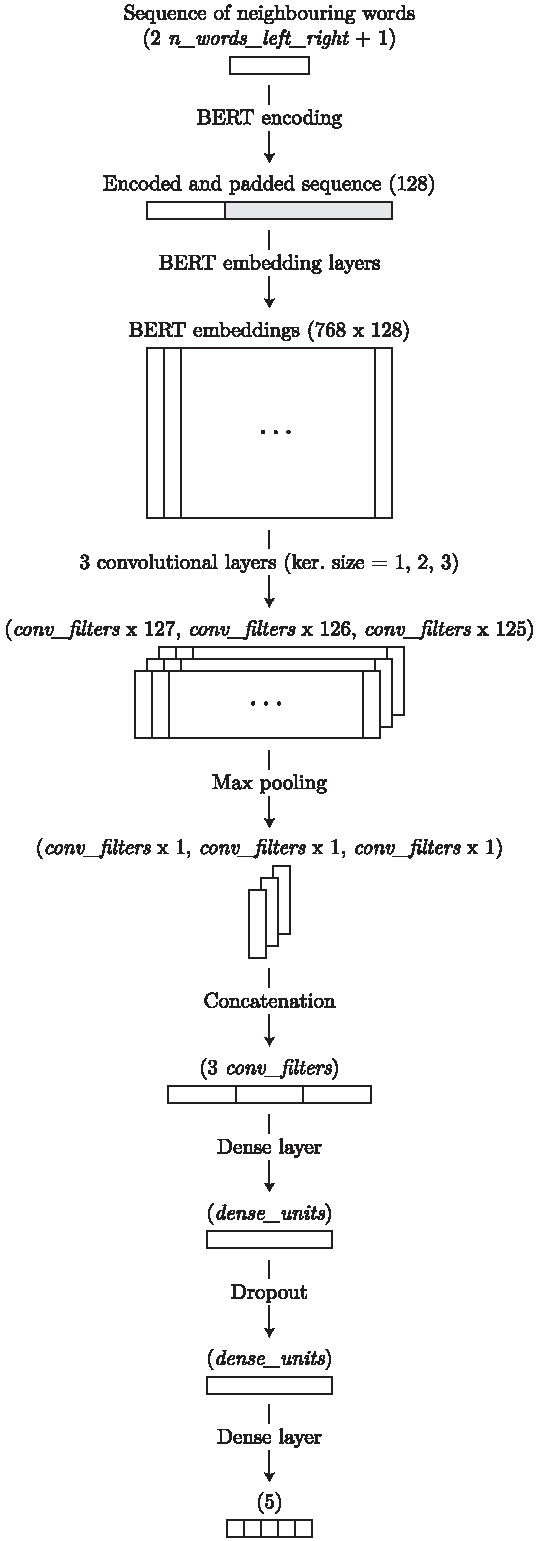
\includegraphics[width=1.0\columnwidth]{bert-model.pdf}
\caption{Architecture of the BERT model.}
\label{fig:bert-model}
\end{figure}

\subsubsection{Further ideas}

TODO (note: following ideas will be used for implementing a few more models)
\begin{itemize}
    \item Current features in the Lex. Feat. model depend mainly on the positive/negative words in the neighborhood of the entity. Instead of looking at the neighborhood, we could use a dependency parser and observe sentiment of the most related words (not necessary in the neighbourhood).
    \item Instead of constructing handcrafted features, we could use BERT model for feature extraction. Those features depend on the context of each word, so we could simply use feature representation of each entity word occurrence and its sentiment as a learning sample for some classifier. With the trained classifier, we could predict sentiment for each occurrence of the entity and calculate the average sentiment for the entity.
    \item Test the effect of using different classifiers (re-implement a single model with different classifiers)
    \item Combine multiple feat. representations into a single model (normalize and concatenate feature vectors from different models and let the classifier use/learn most important features from all models).
\end{itemize}

\subsection{Evaluation}

TODO
\begin{itemize}
    \item 2/3 train, 1/3 test split
    \item Implemented measures: Accuracy, Precision, Recall, F1 score.
\end{itemize}



\section{Results}

TODO

Table~\ref{tab:results} lists the results of our models on the test dataset.

\begin{table}[h]
\centering
\begin{tabular}{lll}
Model            & Accuracy & F1-score \\ \hline
Random model     & 0.203    & 0.128    \\
Majority model   & 0.751    & 0.172    \\
Lexicon Features & 0.756    & 0.197   
\end{tabular}
\caption{Model results on the test dataset.}
\label{tab:results}
\end{table}

\subsection{BERT model}

The model was developed with variety of free parameters.
We tested different configurations in order to see the impact of each parameter on the model performance.
All the results are listed in Table~\ref{tab:bert-results}.

\begin{table}[h]
\centering
\begin{tabular}{lll}
Model            & Accuracy & F1-score \\ \hline
TODO             & TODO     & TODO
\end{tabular}
\caption{TODO.}
\label{tab:bert-results}
\end{table}


\section{Discussion}

TODO



\section{References}

\bibliography{bibliography}
\bibliographystyle{acl_natbib}



\end{document}
